%%%%%%%%%%%%%%%%%%%%%%%%%%%%%%%%%%%%%%%%%%%%%%%%%%%%%%%%%%%%%%%%%%%%%%%%%%%%%%%%
%%%%%%%%%%%%%%%%%%   Vorlage für eine Abschlussarbeit   %%%%%%%%%%%%%%%%%%%%%%%%
%%%%%%%%%%%%%%%%%%%%%%%%%%%%%%%%%%%%%%%%%%%%%%%%%%%%%%%%%%%%%%%%%%%%%%%%%%%%%%%%

% Erstellt von Maximilian Nöthe, <maximilian.noethe@tu-dortmund.de>
% ausgelegt für lualatex und Biblatex mit biber

% Kompilieren mit
% lualatex dateiname.tex
% biber dateiname.bcf
% lualatex dateiname.tex
% lualatex dateiname.tex
% oder einfach mit:
% make

\documentclass[
  tucolor,
  BCOR=12mm,     % 12mm binding corrections, adjust to fit your binding
  parskip=half,  % new paragraphs start with half line vertical space
  open=any,      % chapters start on both odd and even pages
  cleardoublepage=plain,  % no header/footer on blank pages
]{tudothesis}

% \usepackage{geometry}
% \geometry{a4paper, margin=2.5cm, top=3.5cm}
% \usepackage[onehalfspacing]{setspace}

% Warning, if another latex run is needed
\usepackage[aux]{rerunfilecheck}

% just list chapters and sections in the toc, not subsections or smaller
\setcounter{tocdepth}{1}

%------------------------------------------------------------------------------
%------------------------------ Sprache und Schrift: --------------------------
%------------------------------------------------------------------------------
\usepackage{fontspec}
\defaultfontfeatures{Ligatures=TeX}  % -- becomes en-dash etc.

% german language
\usepackage{polyglossia}
\setdefaultlanguage{english}

% for german parts if needed
\setotherlanguages{german}

% intelligent quotation marks, language and nesting sensitive
\usepackage[autostyle]{csquotes}

% microtypographical features, makes the text look nicer on the small scale
\usepackage{microtype}

%------------------------------------------------------------------------------
%------------------------ Für die Matheumgebung--------------------------------
%------------------------------------------------------------------------------

\usepackage{amsmath}
\usepackage{amssymb}
\usepackage{mathtools}

% Enable Unicode-Math and follow the ISO-Standards for typesetting math
\usepackage[
  math-style=ISO,
  bold-style=ISO,
  sans-style=italic,
  nabla=upright,
  partial=upright,
]{unicode-math}
\setmathfont{Latin Modern Math}

% nice, small fracs for the text with \sfrac{}{}
\usepackage{xfrac}


%------------------------------------------------------------------------------
%---------------------------- Numbers and Units -------------------------------
%------------------------------------------------------------------------------

\usepackage[
  locale=DE,
  separate-uncertainty=true,
  per-mode=symbol-or-fraction,
]{siunitx}
\sisetup{math-micro=\text{µ},text-micro=µ}

%------------------------------------------------------------------------------
%-------------------------------- tables  -------------------------------------
%------------------------------------------------------------------------------

\usepackage{booktabs}       % stellt \toprule, \midrule, \bottomrule

%------------------------------------------------------------------------------
%-------------------------------- graphics -------------------------------------
%------------------------------------------------------------------------------

\usepackage{graphicx}
\usepackage{grffile}
\usepackage{subcaption}

% allow figures to be placed in the running text by default:
\usepackage{scrhack}
\usepackage{float}
\floatplacement{figure}{htbp}
\floatplacement{table}{htbp}

% keep figures and tables in the section
\usepackage[section, below]{placeins}


%------------------------------------------------------------------------------
%---------------------- customize list environments ---------------------------
%------------------------------------------------------------------------------

\usepackage{enumitem}

%------------------------------------------------------------------------------
%------------------------------ Bibliographie ---------------------------------
%------------------------------------------------------------------------------

\usepackage[
  backend=biber,   % use modern biber backend
  autolang=hyphen, % load hyphenation rules for if language of bibentry is not
                   % german, has to be loaded with \setotherlanguages
                   % in the references.bib use langid={en} for english sources
]{biblatex}
\addbibresource{references.bib}  % die Bibliographie einbinden
\DefineBibliographyStrings{german}{andothers = {{et\,al\adddot}}}

\usepackage[labelformat=simple]{subcaption}
\renewcommand\thesubfigure{(\alph{subfigure})}

%------------------------------------------------------------------------------
%------------------------------ Sonstiges: ------------------------------------
%------------------------------------------------------------------------------

\usepackage[pdfusetitle,unicode,linkbordercolor=tugreen]{hyperref}
\usepackage{bookmark}
\usepackage[shortcuts]{extdash}
\usepackage{blindtext}

%------------------------------------------------------------------------------
%------------------------------    TIKZ:   ------------------------------------
%------------------------------------------------------------------------------
\usepackage{tikz}
\usetikzlibrary{shapes.geometric, arrows}
\tikzstyle{edge from parent}=[tugreen,thick,draw]
\tikzstyle{feature} = [rectangle, minimum width=2cm, minimum height=1cm,text centered, draw=white, fill=tugreen]
\tikzstyle{class1} = [rectangle, minimum width=1cm, minimum height=0.75cm,text centered, draw=white, text=white, fill=black]
\tikzstyle{class2} = [rectangle, minimum width=1cm, minimum height=0.75cm,text centered, draw=black, fill=white]
\tikzstyle{pil} = [-, thick, color=tugreen, text=tugreen]

%------------------------------------------------------------------------------
%-------------------------    Angaben zur Arbeit   ----------------------------
%------------------------------------------------------------------------------

\author{Kevin Sedlaczek}
\title{Analysis of the Crab Nebula using Photon Stream data collected by FACT}
\date{\today}
\birthplace{Dortmund}
\chair{Lehrstuhl für Experimentelle Physik Vb}
\division{Fakultät Physik}
\thesisclass{Master of Science}
\submissiondate{31. Dezember 2018}
\firstcorrector{Prof.~Dr.~Dr.~Wolfgang Rħode}
\secondcorrector{Prof.~Dr.~Zweitkorrekteur}

% tu logo on top of the titlepage
\titlehead{\includegraphics[height=1.5cm]{logos/tu-logo.pdf}}

\raggedbottom

\begin{document}
\frontmatter
% \input{content/hints.tex}
\maketitle

% Gutachterseite
\makecorrectorpage

% hier beginnt der Vorspann, nummeriert in römischen Zahlen
\thispagestyle{plain}
\section*{\color{tugreen}Abstract}
%
In imaging air Cherenkov astronomy, the cosmic radiation is observed via the
secondary particles it produces in Earth's atmosphere. These high-energy secondary
particles cause the emission of Cherenkov light, which is measured by the
Cherenkov telescopes' optical cameras. From this light, information on the
cosmic radiation can be derived, to learn about the characteristics of the
cosmic sources. The data, Cherenkov telescopes produce, consists of
properties derived from the time series of measured voltages. These properties
strongly depend on the detector's readout hardware. This work focuses on a new
data representation, developed by Sebastian Mueller: the PhotonStream. It
consists of single reconstructed photons and opens new possibilities for
analyses throughout the field of Cherenkov astronomy. In this work, a first analysis of this new data representation is
performed. To do so, openly accessible data of the First G-APD Cherenkov
telescope is used. Alongside the results of origin reconstruction, gamma hadron
separation and energy reconstruction, detailed investigations on the
PhotonStream's properties and differences to the classical approach are
presented.

\section*{\color{tugreen}Kurzfassung}
%
\begin{german}
Die bildgebende atmosphärische Cherenkov Astronomie beschäftigt sich mit der
Untersuchung kosmischer Strahlung über die Sekundärprodukte dieser. Beim
Durchqueren der Atmosphäre entstehen hochenergetische Sekundärteilchen und die
Emission von Cherenkov Licht wird angeregt. Dieses Licht wird von den optischen
Kameras der Cherenkov Teleskope gemessen, um Informationen über die
Eigenschaften dieser Strahlung und ihrer kosmischen Quellen zu sammeln. Die
Daten, die dabei entstehen, stammen aus Spannungszeitreihen der Kamerasensoren
und werden daher stark von den Eigenheiten dieser beeinflusst. Diese Arbeit
beschäftigt sich mit einer neuen Datenrepräsentation, welche von Sebastian
Mueller entwickelt wurde: dem PhotonStream. Diese Repräsentation nutzt die
Möglichkeit, einzelne Photonen aufzulösen, um einen Datensatz aus diesen zu
erstellen, welcher gleichzeitig von der direkten Sensorantwort entkoppelt ist.
Durch die Darstellung von einzelnen Photonen eröffnen sich neue Möglichkeiten
für die Analyse der Daten und das gesamte Feld der Cherenkov Astronomie.
Diese Arbeit stellt eine erste Analyse dieser Daten aus dem
öffentlichen Datensatz des \textit{First G-APD Cherenkov telescope} dar. Neben
den Analyseergebnissen der Quellrekonstruktion, der Gamma Hadron Separation,
sowie der Energieschätzung, werden detaillierte Untersuchungen der
Eigenschaften und Unterschiede dieser neuen Datenrepräsentation präsentiert.
\end{german}

\tableofcontents

\mainmatter
% Hier beginnt der Inhalt mit Seite 1 in arabischen Ziffern
\chapter{Problemstellung und Datensatz}
\nocite{biblatex, siunitx, scikit-learn, Hunter:2007}%

\chapter{Imaging Air Cherenkov Astronomy}

The atmosphere of earth is continously penetrated by radiation from different
sources within our universe. This cosmic radiation is made up of different types
of particles, interacting with the atmosphere in various ways. There are
charged protons and the uncharged neutrinos and photons (gamma rays). Neutrinos
are uncharged, very light fermions, that interact very weakly and are not
detectable by optical telescopes at all. Protons make up the largest number of
particles reaching earths atmosphere. Due to their electric charge, they are
deflected by magnetic fields and therefore lose information on their origin on
the way to earth, making them unsuitable for Cherenkov astronomy.

Cosmic gamma-rays are photons with a very high energy, originating from bright
sources such as active galactic nuclei or nebulae. When such particles intersect
with earth's atmosphere, they move faster than light within that atmosphere due
to their high energy. Particles moving at such speeds through a medium cause,
among the creation of other particles, the emission of bluish photons, the
Cherenkov-light. Cherenkov-light is emitted directly from the moving particle
within a specific angle towards the direction of movement of that primary
particle.
%
\begin{equation}
    \cos(\vartheta) = \frac{1}{n\beta}
    \label{eq:angle_cherenkov}
\end{equation}
%
As \autoref{eq:angle_cherenkov} shows, this angle depends on the index of
refraction $n$ of the medium and the particle's velocity. Due to this emission
angle the light traverses the medium in a cone-shape, when being described from
earth's point of view. By the time it is reaching the ground it thus
illuminates an elliptical area of about $\SI{200}{\meter}$ diameter, depending
on the height of interaction and the primary particle's energy.
This already implicates that the light, although a secondary product of the
cosmic gamma-ray, can be used to reconstruct physical properties of
said gamma-ray. To do so, the flashes of the Cherenkov-light need to
be captured by cameras capable of filming very short time scales (about
$\SI{e-9}{\second}$).

Imaging Air Cherenkov Telescopes (IACTs) are using videos of this light, to
reconstruct properties of the incident cosmic radiation, by analyzing
properties of the measured pictures. By doing so, the atmosphere is used as a very large Cherenkov-detector material.

The three properties of interest are:
\begin{description}[labelsep=3em, align=right]
  \item[source position]{the position of the source of the primary particle on the sky}
  \item[particle type]{the distinction between cosmic gamma rays and other particles like protons or secondary particles like muons}
  \item[particle energy]{the energy of the primary gamma-ray}
\end{description}

\chapter{The First G-APD Cherenkov Telescope}

The First G-APD Cherenkov Telescope \cite{FACT-Design} (FACT) is a IACT protoype located $\SI{2200}{\metre}$ above sea-level on the Canary island of La Palma.
It measures air-shower-photons with a $\SI{9.5}{\meter\squared}$ aperture provided by a segmented imaging-reflector with $\SI{4.889}{\meter}$ focal-length.
Apart from monitoring bright sources of cosmic gamma-rays, like Markarian 421 and Markarian 501, FACT is used for demonstrating and testing the usage of new technologies in the field of IACTs. Giving it its name, FACT uses a novel kind of detector made of so called Geiger-mode avalanche photomultipliers (GAPD). These photomultipliers make up the 1440 pixels of Silicon-Photo-Multipliers (SiPM), FACT uses to sense photons. Each pixel yields about $\SI{0.1}{\degree}$ field-of-view, giving FACT a total field-of-view of $\SI{4.5}{\degree}$. Using SiPMs instead of Photo-Multiplier-Tubes (PMTs) differentiates FACT from other IACTs and gives it special possibilities. SIPMs are very robust, compared to PMTs and can operate in brighter light. This makes continuos observations even during bright moon possible. The SIPMs furthermore have a high photon detection efficiency. With these assets, FACT is well suited for noticing flares and informing other collaborations of such.
%
\begin{figure}
  \centering
  \includegraphics[width=\textwidth]{Plots/fact.jpg}
  \label{fig:fact}
  \caption{The First G-APD Cherenkov Telescope on the Observatory on the Roque des los Muchachos on the island of La Palma. Image by Kevin Schmidt.}
\end{figure}
%

\chapter{Machine Learning and Random forests}
\label{ch:ML}
%
The analysis tasks described in \autoref{ch:iact} make strong use of machine
learning tools to be performed in the most efficient way. There are a lot of
different machine learning techniques that find increasingly many and
successfull applications in modern physics.

\section{Machine learning}
%
Machine learning describes the field of applied statistics that uses computers to learn to solve certain problems. The \textit{learning} is defined by~\cite{mitchell} as: \enquote{A computer program is said to learn from experience $E$ with respect to some class of tasks $T$ and performance measure $P$, if its performance at tasks in $T$, as measured by $P$, improves with experience $E$.} There is a wide variety of different tasks this can be applied to and many performance measures. The most important preposition for well suited problems is the available experience or in this case the amount of data to learn on.

Machine learning aims at solving problems that profit from the computing power
of modern technology but are not the kind of problem to be solved by a typical
program written by a human \cite{goodfellow}. The concept is to try to
reproduce the concept of intelligence within a computer.

\subsection{The Experience}
%
To make a generic machine learning algorithm work for a specific task it has to
be \textit{trained} on data. Just like a human, it needs to be given
information to base a decision on and to be shown how that decision based on
the information is supposed to look. The kind of data suitable for learning
depends on the kind of algorithm to be used and vice versa. Generally, machine
learning algorithms can be divided into \textbf{supervised} and
\textbf{unsupervised} algorithms, but in this work only supervised algorithms
will be used.

Data to derive experience from for supervised algorithms consists of data points
with a certain feature set and a specific label or true value. The datasets for
the \textit{separation} of two classes for example contain a certain feature
set for every data point and a label for the corresponding class each of these
points belongs to. Unsupervised learning therefore aims at learning to predict
a certain target value (or multiple) from a given feature set including this
value. The used learning data in this analysis is provided by simulations, so
that the true values for the machine learning tasks are known.

\subsection{The Task}
%
The task a machine learning algorithm is supposed to do is the solution of a
specific problem in the best possible way. To reach this solution the process
of learning is used but not the task. A machine learning algorithm used to
distinguish between to things is therefore given the task to distinguish two
things rather than to learn to distinguish these two. The three desired tasks
within the analysis of Cherenkov images are the \textit{separation} of
gamma-rays from hadronic cosmic rays, as well as the \textit{estimation} of the
energy and source position of cosmic gamma-rays. The kind of task already
determines what machine learning techniques are best to be used or which ones
don't suit the task and how working architectures have to look. A classification like the separation

\subsection{The Performance Measure}
%
As described above machine learning is about improving on certain tasks.
Therefore it is essential to quantify the performance during but also after the
learning process. This already implicates that performance measures are very
specific to the task. The performance of a classification task is naturally
measured by the \textbf{accuracy} of the model, because it simply describes how
many of the model's outputs are correct. When validating continuous outputs
rather than discrete classifications an accuracy is not appropriate. The
estimation of the energy, e.g., requires a continuous-valued metric.

The models are trained on specific, simulated data but only to be applied on
datasets they have \textit{not} been trained on. Thus, the interesting metrics
are those calculated on datasets complementary to the training data sets,
because they resemble the real use case. To do so, the whole dataset is divided
into a fraction determined for training and a test set on which the metrics can
be calculated. A frequently used method for this is the
\textbf{cross-validation}. The data set is divided into $n$ equaly sized, random
subsamples; $n-1$ samples are used for training whereas the single excluded
sample is used for validation. This is done $n$ times for each one of the
subsamples and the metrics calculated as the mean value of all the single
validations.

\section{Random forests}
%
One of the most frequently used machine learning algorithms and the one used
for the tasks in this analysis is the so called random forest. This is a
supervised learning algorithm based on the so called \textit{decision tree}.

\subsection{Decision Trees}
%
Decision trees classify data points based on consecutive binary decisions. The
decisions are based on the single features of the data point and result in a
point specific result that is being returned. The number of single binary
decisions (also called \textit{leaf}) preceding the final classification is
called \textit{depth} of the tree. Decision trees are trained on labelled data
and determine thresholds for every feature to classify the data point.
%
\begin{figure}[H]
  \centering
  \begin{tikzpicture}[node distance = 3cm, auto]
    \node (f1) [feature] {\texttt{feature\_1}};
    \node (f2) [feature, below of=f1, xshift=-2.4cm] {\texttt{feature\_2}};
    \node (f3) [feature, below of=f1, xshift=2.4cm] {\texttt{feature\_3}};

    \node (c1) [class1, below of=f2, xshift=-1.2cm] {\texttt{class 1}};
    \node (c2) [class2, below of=f2, xshift=1.2cm] {\texttt{class 2}};

    \node (c3) [class1, below of=f3, xshift=-1.2cm] {\texttt{class 1}};
    \node (c4) [class2, below of=f3, xshift=1.2cm] {\texttt{class 2}};

    \draw [pil] (f1) -- node[anchor=east] {$\mathbf{>15}$\;} (f2);
    \draw [pil] (f1) -- node[anchor=west] {\;$\mathbf{\leq15}$} (f3);
    \draw [pil] (f2) -- node[anchor=east] {$\mathbf{<100}$\;} (c1);
    \draw [pil] (f2) -- node[anchor=west] {\;$\mathbf{\geq100}$} (c2);
    \draw [pil] (f3) -- node[anchor=east] {$\symbf{<-\sfrac{\pi}{2}}$\;} (c3);
    \draw [pil] (f3) -- node[anchor=west] {\;$\symbf{\geq-\sfrac{\pi}{2}}$} (c4);
  \end{tikzpicture}
  \caption{Example sketch of a decision tree. The tree decides whether an input data point is of class 1 or class 2. The available features are \texttt{feature\_1}, \texttt{feature\_2} and \texttt{feature\_3}. This decision tree has a depth of 2 and solves the task of a binary separation at each leaf (green boxes). The decision thresholds are written next to the respective connecting lines.}
  \label{fig:tree}
\end{figure}
%
To determine the best decision threshold for each leaf, a performance measure
for the information gain is necessary. For a classification task the required
metric would be the accuracy. The thresholds are thus optimized to get the best
accuracy at the respective leaf. This way the decision tree is build from the
top leaf downwards until a perfect classification is achieved or until a set
maximum depth is reached.

\subsection{Random forests}
%

\chapter{Representing IACT data}
%
IACTs aim at reconstructing the energy, source position and particle type of
cosmic rays via their Cherenkov-light. The Cherenkov-light flashes that are
only nano seconds in duration are measured and can be separated from background
light from stars or ambient light by their brightness and topology within the
camera image. There are different ways to represent air shower data. FACT uses
the so called main-pulse representation, whereas this work focuses on a novel
data format, both of which are described in the following chapter.

\section{The Main-Pulse representation}
%
Data taken by an Imaging-Air-Cherenkov-Telescope
(IACT), like FACT, is usually represented in so called time series.
These time series owe their name to the fact that they represent voltages at the photosensors over time. Within these time series lie so called main-pulses that represent the increased voltage that a charge deposition of an air-shower causes. So by looking for those main-pulses shower events can be found upon the detector noise and ambient light in the camera. Of course, the main-pulses consist of multiple photon signals and noise superposed over time, but in this state they are electric pulses representing the response of very specific hardware. So rather than measuring physical properties, this means that the charge deposit has to be interpretated to be transferred into physics observables, independant of these specifics \textbf{[which ones?]}. Such interpretations always include assumptions of physical and technical kinds. By integrating the charge in one pixel an equivalent of a photon count can be obtained, called the \textit{photon equivalent} (PE). So the first observable in this representation is the PE which corresponds to the best estimate of the number of photons measured per pixel. The photon counts are spatially located by the corresponding pixel they are assigned to. The 1440 pixels of FACT are the determining grid that yield the spatial coordinates of every shower event.

The second observable is the time. When the telescope is triggered and records
data the arrival time of the event is measured via the time information within
the time series. From the time series a quantized timing information per pixel
can be developed by dividing the event into time slices. From this the arrival
time of the photons per pixel can be calculated by averaging. Thus, the arrival
times $t$ per pixel are the second observable of the main-pulse event
representation, besides the photon-equivalents.

\begin{figure}
  \begin{subfigure}{0.475\textwidth}
    \includegraphics[width=1.1\textwidth, page=40]{Plots/cleaning_facttools_pe_20131104_162.pdf}
  \end{subfigure}
  \begin{subfigure}{0.475\textwidth}
    \includegraphics[width=1.1\textwidth, page=40]{Plots/cleaning_facttools_arrival_times_20131104_162.pdf}
  \end{subfigure}
  \caption{The measured observables of the main-pulse representation are shown as scatter plots within the pixels. On the left the distribution of photon-equivalents $c$ of a typical shower event (Crab observation on November, 4th 2013, run 162, event 80) is shown. On the right the arrival times of that event's photons with respect to the mean arrival time in ns are displayed.}
  \label{fig:mainpulse}
\end{figure}

\section{The PhotonStream representation}

The Photonstream representation aims at creating a data format consisting of photons by storing their observed physical properties. So from the measured time series single photons are extracted instead of deriving photon counts in pixels. Each of these photons is assigned an arrival time and pixel, creating a list of arrival times per photon for each pixel. By doing so, a 3-dimensional data set is created, which can be represented in form of so called point clouds (\autoref{fig:event}).
%
\begin{figure}
  \centering
  \includegraphics[width=1.1\textwidth]{Plots/event2.png}
  \caption{Uncleaned event represented by the 3-dimensional point cloud of the Photonstream. Every blue sphere represents a measured photon in the corresponding time slice and pixel.}
  \label{fig:event}
\end{figure}

\chapter{Analysis chain}
%
\section{Parametrization of Events}
%
\section{Image Cleaning on the PhotonStream}
%
\section{Image Cleaning with pixelbased Thresholds}
%
\section{Energy Estimation}
%
\section{Reconstruction of the Source Position}
%
\section{Signal-Background Separation}

\chapter{The FACT Open Crab Sample}
%

\chapter{Results and Performance}
%
\section{Performance of the PhotonStream on Simulations}
%
\section{Performance of the PhotonStream on Data}
%
\section{Evaluation of the image cleaning}
%
\section{Parameters of DBSCAN}
%
\section{Pixelbased Threshold Cleaning on the PhotonStream}
%

\input{content/08_summary.tex}
\input{content/09_conclusion_outlook.tex}
% \input{content/05_results.tex}


\appendix
% Hier beginnt der Anhang, nummeriert in lateinischen Buchstaben
\chapter{Appendix}
\addtocontents{toc}{\protect\setcounter{tocdepth}{-1}}
%
To quantify the mismatches of proton MC simulations and observed data, a random
forest is trained on the feature set, implemented in the \texttt{FeatureStream}, to distinguish the both. Since the
observed data vastly consists of hadron events, for a perfect simulation it
should hardly be possible to distinguish the data sets, while for existing
mismatches, the AUC of the model quantifies those. The ROC curve is shown in \autoref{fig:mcd_roc}. The resulting AUC of
0.7509\,\pm\,0.0025 is very high and therefore represents a good
discrimination. An AUC this large thus indicates strong data MC mismatches.
%
\begin{figure}
  \centering
  \includegraphics[width=\textwidth]{Plots/data_mc/data_mc_separation.pdf}
  \caption{ROC curve for a random forest model discriminating between proton MC simulations and observed data based in the features implemented in the \texttt{FeatureStream}. The resulting AUC of 0.7509\,\pm\,0.0025 is very high and therefore represents a good discrimination. The proton MC simulations are supposed to model the vast majority of observed data, since the hadron flux is dominating. An AUC this large thus indicates strong data MC mismatches.}
  \label{fig:mcd_roc}
\end{figure}
%

\addtocontents{toc}{\protect\setcounter{tocdepth}{0}}


\backmatter
\printbibliography

\cleardoublepage
\input{content/eid_versicherung.tex}
\end{document}
